\documentclass[11pt, handout]{beamer}

\usepackage[T1]{fontenc}
\usepackage[utf8x]{inputenc}
\usepackage[french]{babel} 
\usepackage{amsmath}
\usepackage{lmodern}
\usepackage{xcolor}
\usepackage{graphicx}
\usepackage{pstricks}
\usepackage{caption}
\usepackage{float}
\usepackage{wrapfig}


\usepackage{lmodern}

 %\usepackage[noframe]{showframe}


\usetheme{Singapore}
%\usecolortheme{dolphin}

\usepackage{multicol}
% \setbeameroption{show only notes}
\setbeameroption{show notes}

\usepackage{pgfpages}
\setbeameroption{show notes on second screen}

\setbeamertemplate{navigation symbols}{}

\definecolor{cloneBlue}{rgb}{0.2,0.2,0.698}


\newenvironment{changemargin}[2]{%
  \begin{list}{}{%
    \setlength{\topsep}{0pt}%
    \setlength{\leftmargin}{#1}%
    \setlength{\rightmargin}{#2}%
    \setlength{\listparindent}{\parindent}%
    \setlength{\itemindent}{\parindent}%
    \setlength{\parsep}{\parskip}%
  }%
  \item[]}{\end{list}} 

\newenvironment{noitemize}
{\begin{list}{}{%
\setlength{\labelwidth}{0em}% largeur de la boite englobant l'étiquette
\setlength{\labelsep}{2pt}% espace entre l'entrée de l'item et l'étiquette
\setlength{\leftmargin}{0pt}% marge de gauche
\renewcommand{\makelabel}{\small\color{cloneBlue}{\textbullet}}}}%
{\end{list}}

\newenvironment{minusitemize}
{\begin{list}{}{%
\setlength{\labelwidth}{0em}% largeur de la boite englobant l'étiquette
\setlength{\labelsep}{2pt}% espace entre l'entrée de l'item et l'étiquette
\setlength{\leftmargin}{-15pt}% marge de gauche
\renewcommand{\makelabel}{\small\color{cloneBlue}{\textbullet}}}}%
{\end{list}}


\setbeamersize{text margin left=0.75cm}
\setbeamersize{text margin right=0.75cm}

\title{ \textbf{PIAD 2013}}
\subtitle[\ldots]{Sujet 32 : Semi-supervised Learning Agents%\\[0.5cm]
}

\author{Auteurs : Lan \textsc{Zhou} \and \& \and Matthieu \textsc{Zimmer}\newline Encadrants : Paolo \textsc{Viappiani} \and \& \and Paul \textsc{Weng}}

\institute{Université Pierre et Marie Curie}
\date{14 Mai}
\logo{
\includegraphics[height=6mm]{images/logo.png}}

% \addtobeamertemplate{footline}{\insertframenumber/\inserttotalframenumber}
\addtobeamertemplate{footline}{\hfill\insertframenumber/\inserttotalframenumber}

%%%%%%%%%%%%%%%%%%%%%%%%%%%%%%%%%%%%%%%%%%%%%%%%%%%%%%%%%%%%%%%%%%%%%%%%%%%%%%%%%%%%%%%%%%%%%%%%%%%%%%%%




\begin{document}

% \usebackgroundtemplate{
% \begin{picture}(200,200)
% \put(5, 60){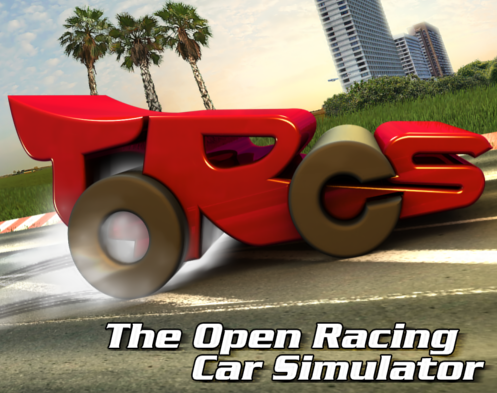
\includegraphics[width=100px]{images/torcs.png}}
% \end{picture}
% }

\begin{frame}
\maketitle
\end{frame}

\note{
L'apprentissage semi-supervisé
}


\usebackgroundtemplate{}
\begin{frame}

\begin{center}{\Large Plan }\end{center}
  \tableofcontents
\end{frame}

\note{

\begin{itemize}
 \item et ce qu'on propose dans notre bibliothèque
 \item quelques algorithmes sarsa , qlearning
 \item Mise en pratique
\end{itemize}


}
% 
% \usebackgroundtemplate{
% \begin{picture}(200,300)
% \put(220, 50){\includegraphics[width=90px]{images/embryo.jpg}}
% \end{picture}
% }
% 


\begin{frame}
 \frametitle{Introduction}
 \framesubtitle{Problématique}
 2 grande classe d'apprentissage :
 \begin{itemize}
  \item Apprentissage supervisé
  \item Apprentissage non supervisé
 \end{itemize}
 --> apprentissage semi-supervisé <--\\[1cm]
 
 Objectifs :
 \begin{itemize}
  \item Developper bibliothèque
  \item Liaison simulateur
 \end{itemize}

 
 
\end{frame}
\usebackgroundtemplate{}

\note{ 
Réseau de neurones, ...

Parfois les agents apprendrons d'eux meme, quelques fois du superviseur

Implémentation C++

Pour arriver à un apprentissage semi supervisé, nous allons partir d'un apprentissage non supervisé
: l'APR. Lan va donc vous introduire aux notions de bases.
}


\section{Théorie}



\subsection{Processus de décision Markovien}

\begin{frame}
 \frametitle{Processus de décision Markovien}
%  \framesubtitle{}

 


  \begin{minipage}{0.5\textwidth}
 \begin{flushleft}
 \begin{itemize}
  \item Ensemble d'États
  \item Ensemble d'Actions
  \item Matrice transition
  \item Fonction de récompense
 \end{itemize}
  \end{flushleft}
 \end{minipage}
 ~
 \begin{minipage}{0.4\textwidth}
 \begin{flushright}
  \begin{figure}
      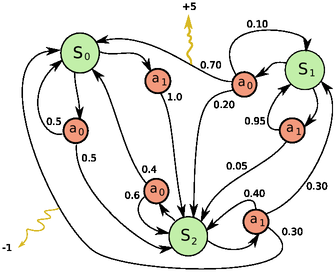
\includegraphics[height=4cm]{images/MDP.png} \\
  \end{figure}
  \end{flushright}
 \end{minipage}
 
 
  Maximiser un critère $ \pi^* \in \operatorname{argmax} = E^{\pi}[r_0 + {\gamma}r1 + {\gamma}^2r_2 + ... ]$
  \newline \hspace*{5.6cm}$ = E^{\pi}[ \sum \limits_{t=0}^\infty {\gamma}^tr_t]$
 
\end{frame}

\note{
Un agent
\newline
Les résultats des actions sont indéterminées
\newline
Pour finir, le problème revient à trouver une politique qui maximise l'espérance des récompenses.
}

\subsection{Apprentissage par Renforcement}

\begin{frame}
 \frametitle{Apprentissage non supervisé}
 \framesubtitle{Apprentissage par Renforcement}

  
  \begin{minipage}{0.4\textwidth}
    \begin{flushleft}
    Algorithmes 
      \begin{itemize}
	\item Sarsa
	\item Q-Learning
      \end{itemize}
    \end{flushleft}
  \end{minipage}
    ~ 
    \begin{minipage}{0.4\textwidth}
    \begin{flushright}
       Q = Etat x Action
      \end{flushright}
    \end{minipage}


    \begin{figure}
  \begin{center}
 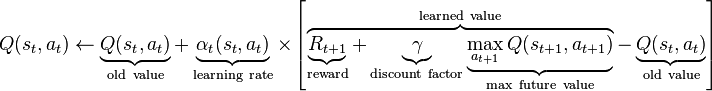
\includegraphics[height=1.5cm]{images/qlearnupd.png} \\
 \end{center}
  \end{figure}
 
\end{frame}

\note{
On s'est concentré sur 2 grands algorithmes : SARSA \& Q-Learning
que nous avons implémenté dans notre bibliothèque

Les 2 utilisent un tableau Q qui permet de facilement retrouver
la meilleur action pour un état donné

La formule de mise à jour durant l'apprentissage est la suivante 

}


\begin{frame}
 \frametitle{Apprentissage par Renforcement}
 \framesubtitle{Prendre en compte l'historique}

     \begin{figure}
    \begin{center}
 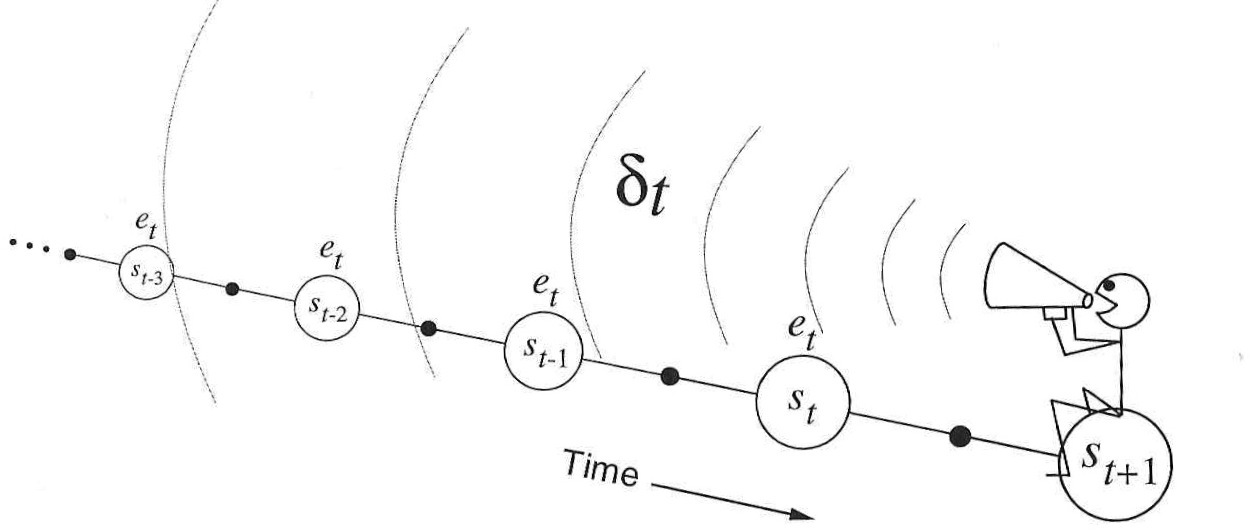
\includegraphics[height=3cm]{images/histo.jpeg} 
 \end{center}
  \end{figure}


      Trace
          \begin{figure}
 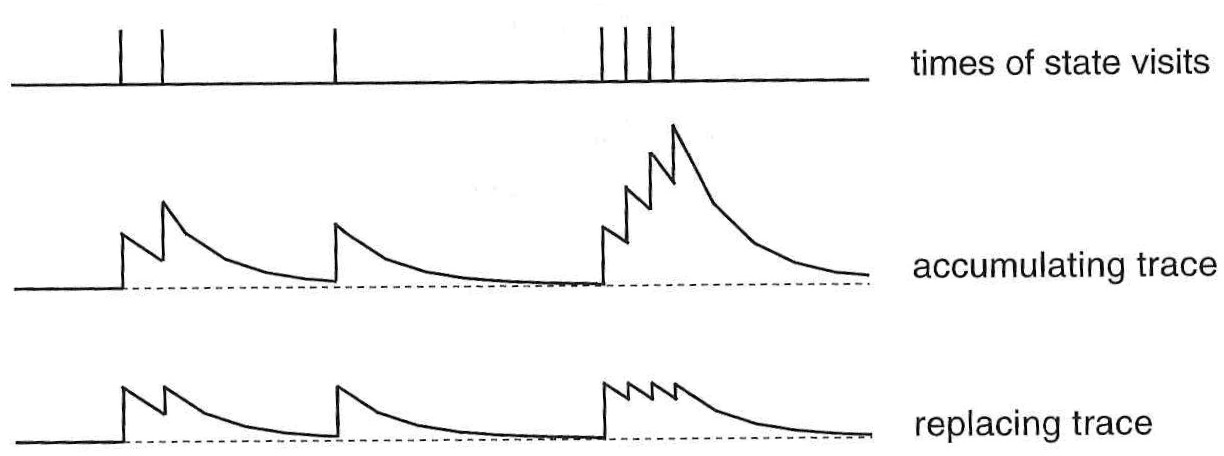
\includegraphics[height=3cm]{images/trace.jpeg}
  \end{figure}

\end{frame}

\note{
Un des problèmes de la version précédente est qu'il n'y a pas de notion d'historique.

Si je fais une erreur ou quelques choses de bien maintenant, c'est uniquement grâce à 
ma dernière action. Ca prolongue beaucoup la phase d'apprentissage.


Mais ça ne suffit toujours pas.
}

\begin{frame}
 \frametitle{Fonction d'approximation}
 \framesubtitle{Descente de gradient}
 
   \begin{minipage}{0.4\textwidth}
    \begin{flushleft}
 Pourquoi? 
 \begin{itemize}
  \item Mémoire
  \item Temps d'apprentissage
 \end{itemize}
    \end{flushleft}
  \end{minipage}
    ~ 
    \begin{minipage}{0.4\textwidth}
    \begin{flushright}
       $Q(s,a) = \sum\limits_{i=1}^n \theta_{i} \times f_{i}(s,a)$
 
      \end{flushright}
    \end{minipage}
 

          \begin{figure}
 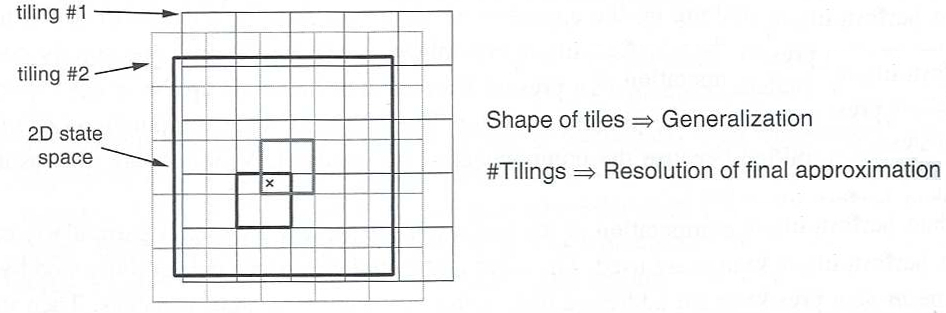
\includegraphics[height=3cm]{images/tiling.jpeg}
  \end{figure}
 
\end{frame}

\note{
l'apprentissage par renforcement «de base» n'est pas extensible à très grand espace d'état, 
car il faut maintenir dans la mémoire très grandes matrices

On va donc chercher maintenant à approximer Q(s,a) par cette fonction.
On notera que les états ne sont alors plus discrétisés.

On gagne en mémoire, plus qu'on tableau teta, et en généralisation, ce qu'il apprend dans
une configuration il peut le généraliser.


Voici qui clos la partie sur l'APR.
}



\begin{frame}
 \frametitle{Semi supervisé}
 
  3 idées 
  \begin{itemize}
   \item Agir sur les récompenses
   \item Agir sur le choix des actions
   \item Agir sur la stratégie (exploitation/exploration)
  \end{itemize}

 
\end{frame}


\note{
Comment intégrer une supervision?\newline
Un tuteur va surveiller l'agent de temps en temps et complémenter la fonction de récompense
\newline contrôler l'agent

}


\begin{frame}
  \begin{center}{\Large Plan }\end{center}
  \tableofcontents
\end{frame}

\note{
Nous passons donc maintenant à la mise en pratique et à la liaison avec le simulateur.
}


\section{Pratique}

\subsection{TORCS}


\usebackgroundtemplate{
\begin{picture}(200,350)
\put(2, 78){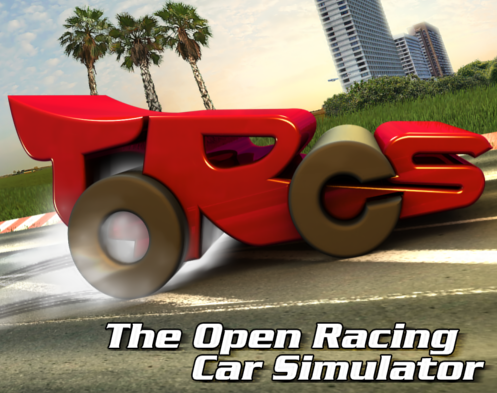
\includegraphics[width=100px]{images/torcs.png}}
\end{picture}
}

\begin{frame}
 \frametitle{TORCS}
 
\begin{center}
  \begin{figure}
      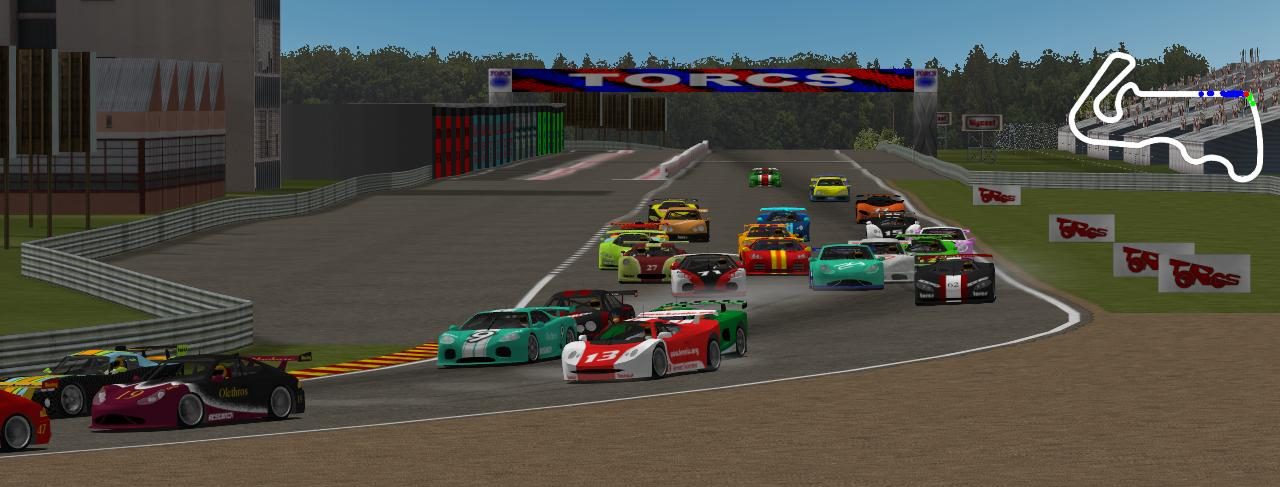
\includegraphics[height=4cm]{images/torcs2.jpg} \\
  \end{figure}
\end{center}
 \vfill
\end{frame}
\usebackgroundtemplate{}

\note{
Le simulateur que nous avons choisi avec nos encadrants est TORCS.

Il permet de simuler des courses de voitures en 3D pour faire
de jolies démos.

Il est open-source et écris en C/C++, très personnalisable,
il permet d'intégrer des modules indépendants pour les agents.

Il permet également d'être simuler sans GUI pour que les agents puissent apprendre.
}

\begin{frame}
 \frametitle{Les entrées}
  
  
  \begin{minipage}{0.5\textwidth}
 \begin{flushleft}
 Capteurs locaux -> généralisation des pistes
 \begin{itemize}
  \item distance au centre 
  \item angle tangent
  \item vitesse
  \item longueur segment
  \item angle prochain virage
 \end{itemize}
  \end{flushleft}
 \end{minipage}
 ~
 \begin{minipage}{0.4\textwidth}
 \begin{flushright}
  \begin{figure}
      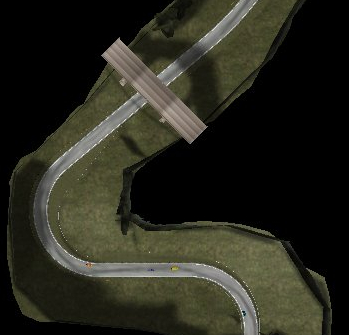
\includegraphics[height=4cm]{images/track.jpg} \\
  \end{figure}
  \end{flushright}
 \end{minipage}

\end{frame}

\note{

[Utiliser l'image]

}

\begin{frame}
 \frametitle{Les actions}

   \begin{minipage}{0.4\textwidth}
 \begin{flushleft}
 \begin{itemize}
  \item Direction
  \item Freinage
  \item Acceleration
  \item Boîte vitesse
 \end{itemize}
  \end{flushleft}
 \end{minipage}
 --- >
 \begin{minipage}{0.4\textwidth}
 \begin{flushright}
 \begin{itemize}
  \item Direction
  \item Vitesse (4 valeurs)
 \end{itemize}
  \end{flushright}
 \end{minipage}
 
\end{frame}

\note{
Dans TORCS il y a en 4 actions possible, qu'on a fusionné en 2 pour simplifier le problème.


Le calcul du changement de boîte à vitesse est automatique.

4 valeurs : acc, ne rien faire,  freiné, reculé.
}

\begin{frame}
 \frametitle{Les récompenses}
  
  
  
\begin{minipage}{0.5\textwidth}
 \begin{flushleft}
Sur route et avance : 
\begin{itemize}
 \item vitesse $\in [100;6000]$
\end{itemize}

Avance pas : - 500 

Avance dans un mur : -1000

Bloqué et Recule : 15

Sens inverse
\begin{itemize}
 \item vitesse $\in [-4000;-2000]$
\end{itemize}

Sort de route 
\begin{itemize}
 \item écart $\in [-1000;-4000]$
\end{itemize}

  \end{flushleft}
 \end{minipage}
 ~
 \begin{minipage}{0.4\textwidth}
 \begin{flushright}
  \begin{figure}
      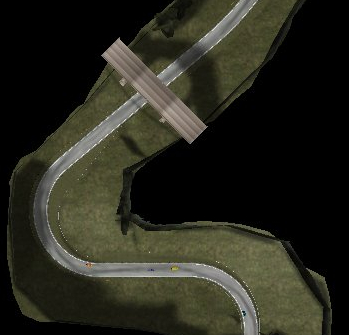
\includegraphics[height=4cm]{images/track.jpg} \\
  \end{figure}
  \end{flushright}
 \end{minipage}
\end{frame}

\note{

}

\begin{frame}
 \frametitle{Demo}

 + Quelques stats

\end{frame}

\note{
L'autre objectif du projet était d'intégrer des feedbacks d'un superviseur à TORCS.
}

\subsection{Feedbacks} 

\begin{frame}
 \frametitle{Mode superviseur}


 Agir sur les récompenses

\end{frame}

\note{
L'autre objectif du projet était d'intégrer des feedbacks d'un superviseur à TORCS.
}

\begin{frame}
 \frametitle{Mode contrôle}

 Agir sur les actions\\
 Montrer à l'agent comment conduire
 Démo

\end{frame}

\note{
Merci aux encadrants, ...
}




\section{}

\begin{frame}
 \frametitle{Conclusion}
 \framesubtitle{Aller plus loin...}
 
 \begin{itemize}
 \item 
 \end{itemize}
 
\end{frame}

\note{
Merci de nous avoir écouté.
}


\begin{frame}
 \frametitle{References \& Remerciements}

%  Livre : 
 \begin{itemize}
  \item Reinforcement Learning : An Introduction, 1998
  \newline Sutton, Richard S and Barto, Andrew G 
  \item Image Wikipédia : Apprentissage par renforcement
 \end{itemize}

\end{frame}



\end{document}


